% Qualitative visual-input comparison
\begin{figure}[t]
  \centering
  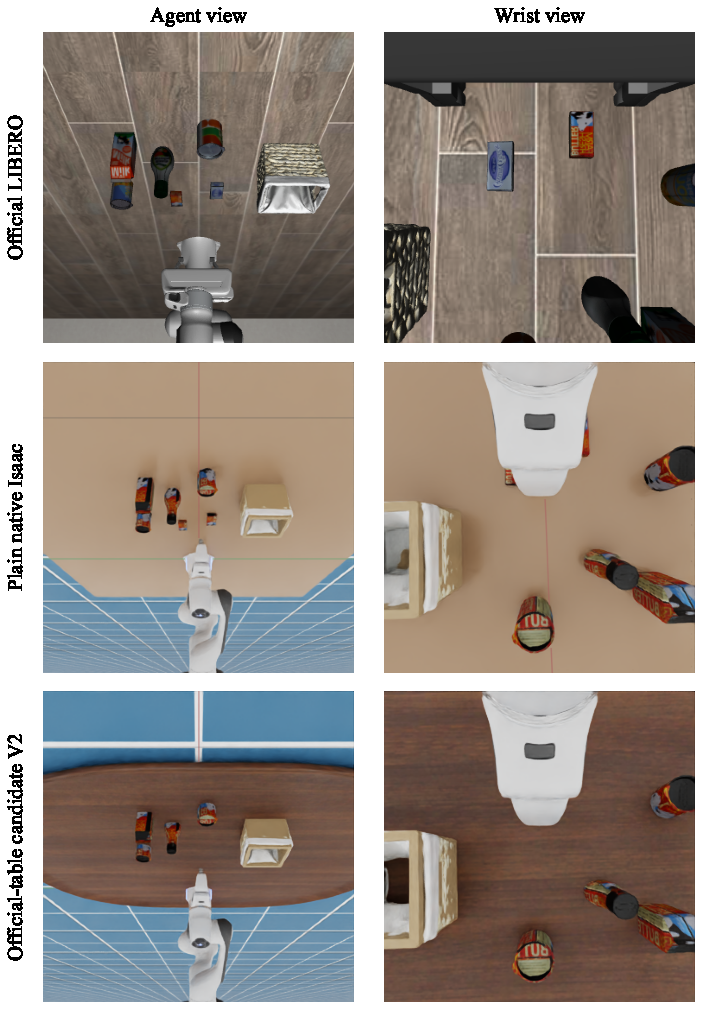
\includegraphics[width=0.95\textwidth]{outputs/xvla_isaac_visual_canary_v1/visual_input_comparison.pdf}
  \caption{Policy inputs for the same task, reset seed, and instruction. The top row is the official LIBERO reference observation; the lower rows are plain and official-table V2 native-Isaac reset renders under the same native state contract. V2 restores a wood surface but retains table-extent, lighting, and robot-appearance mismatch.}
  \label{fig:xvla-isaac-visual-inputs}
\end{figure}

% First action-chunk comparison
\begin{figure}[t]
  \centering
  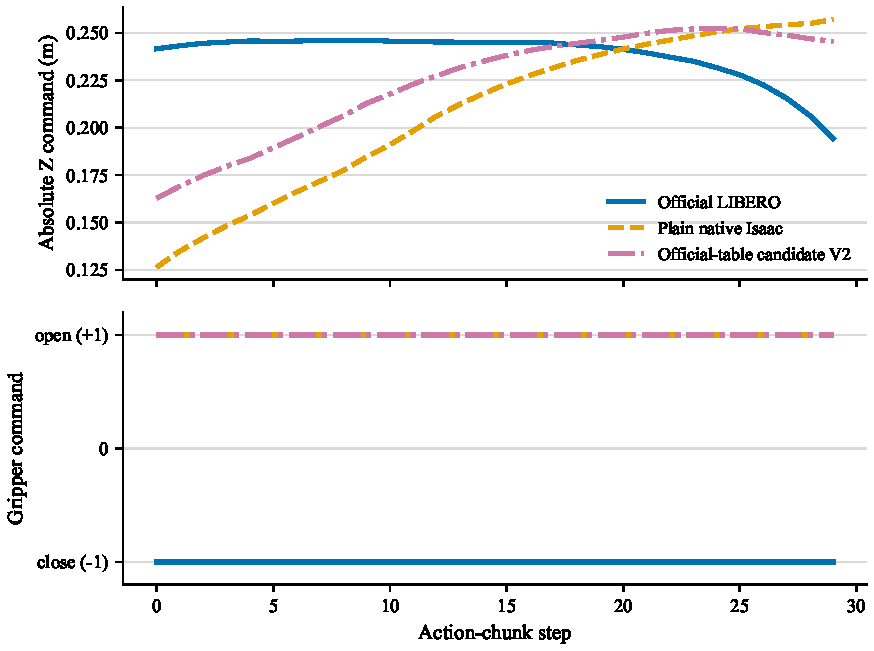
\includegraphics[width=0.75\textwidth]{outputs/xvla_isaac_visual_canary_v1/first_chunk_action_comparison.pdf}
  \caption{Mean X-VLA first action chunk across three paired inference seeds, with official robot state held fixed within each official-vs-native image pair. The table candidate partially recovers the Z command but retains the opposite gripper sign throughout the chunk. This is not task-success evidence.}
  \label{fig:xvla-isaac-first-chunk}
\end{figure}
